% Przegląd literatury i ogólnie pojęty research
\documentclass[a4paper,12pt]{article}
\usepackage[polish]{babel}
\usepackage[utf8]{inputenc}
\usepackage[T1]{fontenc}
\usepackage{indentfirst}
\usepackage[top=2.5cm, bottom=2.5cm, left=2.5cm, right=2.5cm]{geometry}
\usepackage{amsmath}
\usepackage{hyperref}
\usepackage{graphicx}

\title{Symulacja ruchu drogowego na IV obwodnicy Krakowa}
\author{Szymon Gałuszka, Michał Worsowicz, Maciej Nalepa}
\date{\today}
\begin{document}
	\maketitle
	
	\section{Wprowadzenie}
	
	Symulacja ruchu pozwala znaleźć przyczny utrudnienia ruchu, a tym samym poprawić jakość budowania dróg. Jest ona nierozłącznym narzędziem przy projektowaniu i planowaniu nowych tras i skrzyżowań. Dzięki symulacji można przewidzieć zachowanie pojazdów na przyszłych jezdniach; sprawdzić, czy poradzą sobie z oczekiwanym natężeniem ruchu oraz upewnić się, czy proponowane rozwiązanie nie wywoła kolejnych, nieprzewidzianych utrudnień.
	
	W ostatnich latach, zarówno w Polsce jak i na świecie, nastąpił rozwój inteligentnych systemów kontroli ruchu ulicznego, które wykorzystują wiele rodzajów danych - zbieranych za pomocą odpowiednich czujników i systemów - aby w  odpowiedni sposób zarządzać sygnalizacją świetlną na skrzyżowaniach i optymalizować przepływ ludzi podróżujących np. samochodem, rowerem lub pieszo.
	
	Jednak historia symulacji ruchu ulicznego sięga wiele lat wcześniej. Pierwsze modele natężenia ruchu ulicznego pojawiły się już w latach pięćdziesiątych wraz z rosnącym dostępem do pierwszych komputerów. Rosnąca moc obliczeniowa pozwoliła w następnych latach opracowywać coraz bardziej skomplikowane i zaawansowane modele, które uwzględniały wiele zmiennych oraz różniły się od siebie założeniami i sposobami implementacji. Możemy je podzielić na dwa typy: mikro- i makroskopijne. Pierwszy rodzaj modeli symuluje pojedyńcze jednostki, np. samochody, gdzie każda z nich jest reprezentowana przez swoje parametry, takie jak obecna prędkość lub pozycja. Drugi typ modeli - makroskopijny - uwzględnia natomiast zależności pomiędzy właściwościami natężenia ruchu takimi jak gęstość, przepustowość, średnia prędkość ruchu na drodze. Są tu integrowane mikroskopijne modele, ale w sposób, który przekształca charakterystyki z poziomu pojedyńczych jednostek na porównywalne dla całego systemu. Aby w miarodajny sposób przeprowadzić symulację ruchu drogowego w danym terenie, będzie należało wybrać odpowiedni sposób na realizację rozwiązania problemu.
	
	\section{Definicja problemu}
	
	Nasz cel to symulacja ruchu drogowego na IV obwodnicy Krakowa \ref{obw}. 
	Konieczna jest definicja tras oraz sposobu poruszania się po nich.
	Na obwodnicy nie ma sygnalizacji świetlnej, skrzyżowania znajdują się najczęściej pod wiaduktem i najpierw należy zjechać z drogi szybkiego ruchu.
	Trasa ma zróżnicowane ograniczenia prędkości oraz różną ilość pasów ruchu.
	
	Ruch drogowy powinien uwzględniać pojazdy osobowe, ciężarowe i transport publiczny.
	Ciężkie pojazdy obowiązują inne ograniczenia prędkości oraz zajmują więcej przestrzeni na jezdni.
	Napływ ruchu powinien odbywać się przez wjazdy na obwodnicę, które wpuszczają samochody z określoną częstotliwością,która może zależeć od pory dnia.
	
	Koniecznym elementem jest symulacja zmiany pasa ruchu. 
	Symulacja może obejmować wydarzenia losowe, takie jak:
	
	\begin{itemize}
		\item blokada pasa ruchu,
		\item zamknięcie zjazdu,
		\item nagłe hamowanie.
	\end{itemize}

	Można rozszerzyć mapę dla zakończonej obwodnicy, która aktualnie jest w planach.
	
	\begin{figure}
		\label{obw}
		\centering
		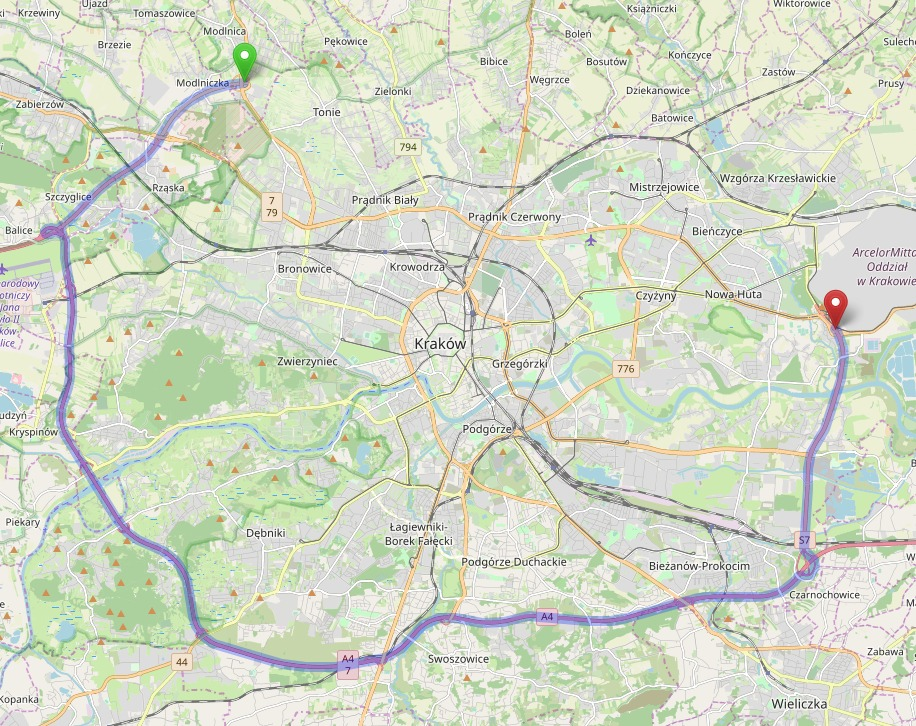
\includegraphics[width=0.7\textwidth]{openstreet.jpg}
		\caption{Obwodnica IV na mapie (2019) \cite{map}.}
	\end{figure}
	
	\section{Propozycja rozwiązania}
		
	W celu rozwiązania zadanego problemu należy oprzeć badania na odpowiednim modelu, który to pozwoli nam zasymulować ruch drogowy. Bardzo dobrym przykładem takiego szablonu jest model Nagela-Schreckenberga, który to zdecydowaliśmy się wykorzystać.
	
	Model Nagela-Schreckenberga to teorytyczny model mikroskopowy o charakterze dyskretnym, w którym droga podzielona jest na komórki. Każda z komórek interpretowana jest na jeden z dwóch sposobów:
	
	\begin{itemize}
		\item fragment pustej drogi,
		\item fragment zawierający pojedyńczy samochód
	\end{itemize}

	Każdy samochód $n$ posiada swoją prędkość $v(n)$ o wartości liczby naturalnej, nie większej od prędkości maksymalnej $v_{max}$ (symbolizuje ona ograniczenie prędkości na drodze).
	Czas $t$ w modelu Nagela-Schreckenberga przyjmuje wartość dyskretną o stałym kroku, gdzie każdy etap można podzielić na cztery następujące po sobie czynności:
	
	\begin{enumerate}
		\item Przyspieszanie: \\
		Jeżeli $v(n) < v_{max}$ to prędkość samochodu może ulec zwiększeniu o zadaną jednostkę, nie przekraczając prędkości maksymalnej.
		\item Zwalnianie: \\
		Jeżeli odległość $d(n)$ samochodu $n$ od samochodu znajdującego się przed nim jest mniejsza od prędkości $v(n)$ tego samochodu to prędkość samochodu ulega zmniejszeniu. Jako że odległość mierzona jest w liczbie komórek, a prędkość w liczbie komórek na jednostkę czasu, to prędkość ostateczna może wynosić maksymalnie $d(n)$ na jednostkę czasu, a minimalnie zero.
		\item Losowość: \\
		Czynność ta symbolizuje wszelkie przypadki losowe z jakimi kierowca może spotkać się na drodze. Dla każdego samochodu $n$, gdzie $v(n) > 0$, prędkość zostaje zmniejszona o jedną jednostkę, z pewnym zadanym prawdopodobieństwem $p$.
		\item Ruch samochodu: \\
		W ostatnim kroku każdy z samochodów zostaje przesunięty do przodu o odpowiednią ilość komórek, wynikającą z jego prędkości.
	\end{enumerate}

	Implementacja zostanie wykonana w języku Python ze względu na łatwość obsługi i dużą dostępność modułów oraz rozszerzeń.
	
	\pagebreak
	\begin{thebibliography}{15}
		\bibitem{oneroad}
		One Road, \textit{Symulacje ruchu drogowego},
		\texttt{\href{http://www.oneroad.pl/symulacje-ruchu-drogowego/}{oneroad.pl}}
		
		\bibitem{wikikrk}
		Wiki, \textit{Kraków Obwodnica IV},
		\texttt{\href{https://pl.wikipedia.org/wiki/Obwodnice_Krakowa\#IV_obwodnica}{wikipedia.org}}
		
		\bibitem{map}
		OpenStreet, \textit{mapa},
		\texttt{\href{https://www.openstreetmap.org/}{openstreetmap.org}}
		
		\bibitem{nagel}
		K. Nagel, M. Schreckenberg, \textit{Two lane traffic simulations using cellular automata},
		\texttt{\href{https://arxiv.org/pdf/cond-mat/9512119.pdf}{arxiv.org}}
		% https://www.sciencedirect.com/science/article/pii/0378437195004424
		
		\bibitem{trends}
		Andreas Pell, \textit{Trends in Real-time Traffic Simulation},
		\texttt{\href{https://www.sciencedirect.com/science/article/pii/S2352146517304684}{sciencedirect.com}}
		
		\bibitem{wikitraffic}
		Wiki, \textit{Traffic simulation},
		\texttt{\href{https://en.wikipedia.org/wiki/Traffic_simulation}{wikipedia.org}}
	\end{thebibliography}
	
\end{document}
